\documentclass{article}

\usepackage{graphicx}
\usepackage{tikz}
\usepackage{tikzsymbols}
\usetikzlibrary{calc,patterns,shapes.geometric}
\pagestyle{empty}
\usepackage[margin=0pt]{geometry}
\geometry{papersize={14in,12in}}

\def\centerarc[#1](#2)(#3:#4:#5){\draw[#1] ($(#2)+({#5*cos(#3)},{#5*sin(#3)})$) arc (#3:#4:#5);}

\begin{document}
	\begin{figure}
		\centering
		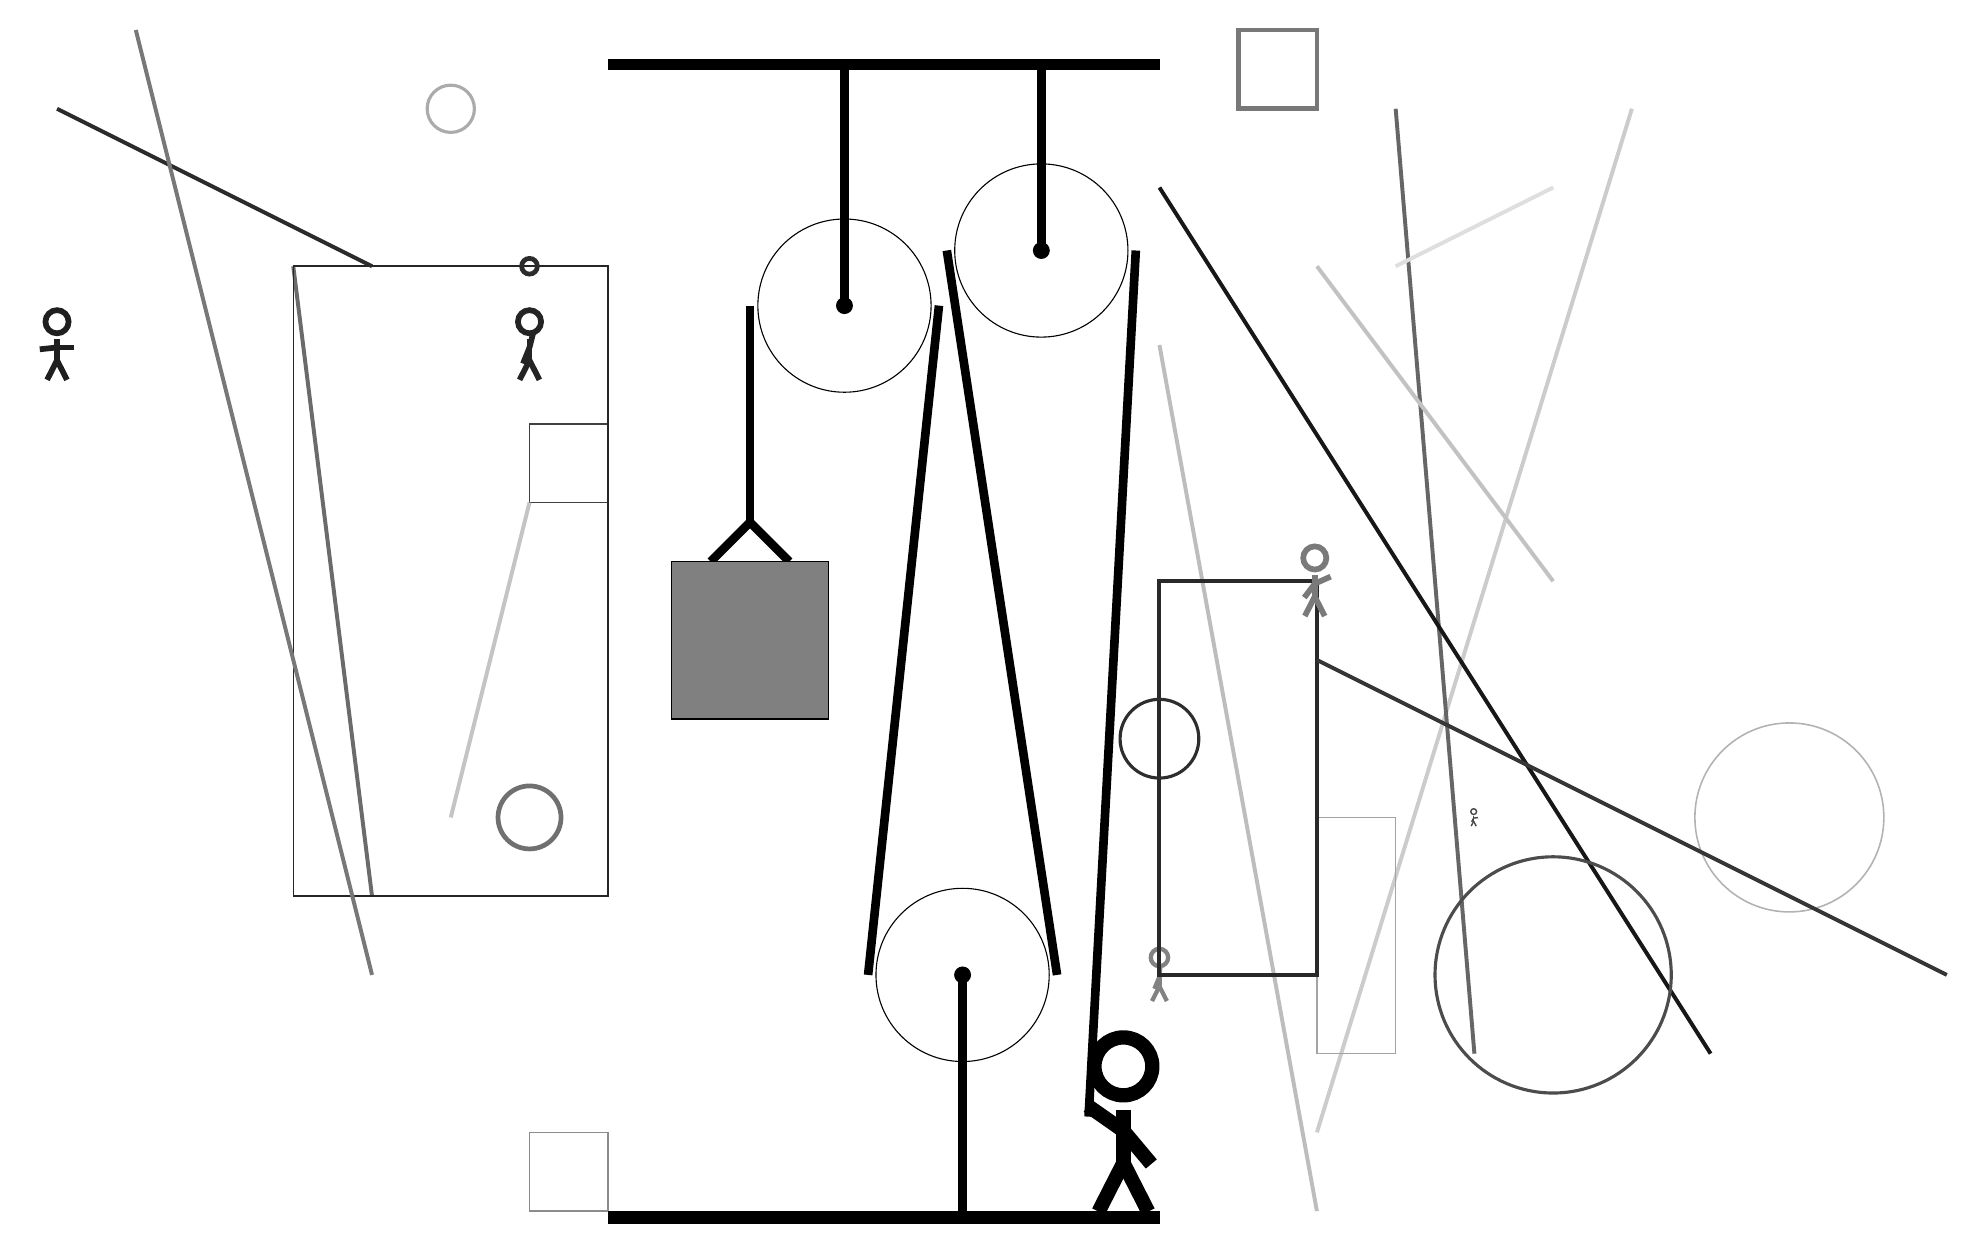
\begin{tikzpicture}
			%%%%% START %%%%%
			
			\draw[fill=black] (-2, 11.5) rectangle (5, 11.625);
			
			\draw (1, 8.5) circle (1.1);
			\draw[fill=black] (1, 8.5) circle (0.1);
			\draw[line width=1.1mm]  (1, 11.5) -- (1, 8.5);
			
			\draw[line width=0.2mm, color=black!45] (-2, -2) rectangle (-3, -3);
			
			\draw[line width=0.5mm, color=black!58](-5, 1) -- (-6, 9);
			\draw[line width=0.5mm, color=black!20](7, -2) -- (11, 11);
			\draw [line width=0.6mm, color=black!56](-3, 2) circle (0.4);
			\draw [line width=0.2mm, color=black!30](13, 2) circle (1.2);
			\draw[line width=0.5mm, color=black!26](5, 8) -- (7, -3);
			\draw[line width=0.2mm, color=black!75] (-2, 6) rectangle (-3, 7);
			\draw[line width=0.2mm, color=black!85] (-2, 1) rectangle (-6, 9);
			\draw[line width=0.5mm, color=black!60](9, -1) -- (8, 11);
			
			\draw[line width=0.5mm, color=black!83](-5, 9) -- (-9, 11);
			\node[line width=0.2mm, color=black!88] at (-9, 8) {\Strichmaxerl[4][6][0]};
			
			\node[line width=0.7mm, color=black!86] at (-3, 8) {\Strichmaxerl[4][68][76]};
			\draw[line width=0.5mm, color=black!91](5, 10) -- (12, -1);
			
			\draw[line width=0.2mm, color=black!36] (7, -1) rectangle (8, 2);
			\draw[line width=0.5mm, color=black!24](10, 5) -- (7, 9);
			\draw[line width=0.5mm, color=black!13](8, 9) -- (10, 10);
			
			\node[line width=0.2mm, color=black!49] at (5, 0) {\Strichmaxerl[3][67][85]};
			\draw[line width=0.5mm, color=black!84] (7, 5) rectangle (5, 0);
			\draw [line width=0.4mm, color=black!82](5, 3) circle (0.5);
			\draw [line width=0.4mm, color=black!33](-4, 11) circle (0.3);
			\draw [line width=0.4mm, color=black!70](10, 0) circle (1.5);
			\draw [line width=0.6mm, color=black!83](-3, 9) circle (0.1);
			\draw[line width=0.5mm, color=black!23](-4, 2) -- (-3, 6);
			\draw[line width=0.5mm, color=black!79](7, 4) -- (15, 0);
			\node[line width=0.6mm, color=black!72] at (9, 2) {\Strichmaxerl[1][62][6]};
			
			\node[line width=0.5mm, color=black!52] at (7, 5) {\Strichmaxerl[4][53][24]};
			
			\draw[line width=0.6mm, color=black!53] (7, 11) rectangle (6, 12);
			\draw[line width=0.5mm, color=black!53](-5, 0) -- (-8, 12);
			
			\draw[fill=white](2.5, 0.0) circle (1.1);
			\draw[fill=black] (2.5, 0.0) circle (0.1);
			\draw[line width=1.1mm]  (2.5, -3) -- (2.5, 0.0);
			
			\draw[fill=white](3.5, 9.2) circle (1.1);
			\draw[fill=black] (3.5, 9.2) circle (0.1);
			\draw[line width=1.1mm] (3.5, 11.5) -- (3.5, 9.2);
			
			\draw[line width=1.1mm] (-0.7, 5.25) -- (-0.2, 5.75) -- (0.3, 5.25);
			\draw[fill=black!50] (-1.2, 5.25) rectangle (0.8, 3.25);
			
			\draw[line width=1.1mm] (-0.2, 8.5) -- (-0.2, 5.75);
			\centerarc[line width=1.1mm](1, 8.5)(0:180:1.2000000000000002);
			\draw[line width=1.1mm](2.2, 8.5) -- (1.3, 0.0);
			\centerarc[line width=1.1mm](2.5, 0.0)(180:360:1.2000000000000002);
			\draw[line width=1.1mm](3.7, 0.0) -- (2.3, 9.2);
			\centerarc[line width=1.1mm](3.5, 9.2)(0:180:1.2000000000000002);
			\draw[line width=1.1mm](4.7, 9.2) -- (4.1, -1.8);
			
			\node at (4.5, -1.9) {\Strichmaxerl[10][-35][-50]};
			
			\draw[fill=black] (-2, -3) rectangle (5, -3.15);
			
			%%%%% END %%%%%
		\end{tikzpicture}
	\end{figure}	
\end{document}